\section{Introduction}
%%%%%%%%%%%%%%%%%%%%%%%%%%%%%%%%%%%%%%%%%%%%%%%%%%%%%%%%%%%%%%%%%%%%%%%%%%%%%%%%
\hl{This report outlines the}
%%%%%%%%%%%%%%%%%%%%%%%%%%%%%%%%%%%%%%%%%%%%%%%%%%%%%%%%%%%%%%%%%%%%%%%%%%%%%%%%
\subsection{Motivation: The problem we are solving}\label{sec:problem}
Benchtop power supplies are an essential tool for electrical engineers, they provide a DC voltage that can be varied by the user within a fixed range. It is an important tool during the design phase of a project when the debugging and evaluation of hardware is occurring. Due to the increasing complexity of embedded systems, there are naturally more integrated circuits present in hardware and all of which may require different voltages to operate. There is also a shift to reduce the power requirements of devices hence being able to assess the viability of a system at low voltages requires a variable voltage source. It is an important step to be able to generate voltages to power the systems and test each individual element separately before the power system has been completely designed and integrated. 
\begin{figure}
    \centering
    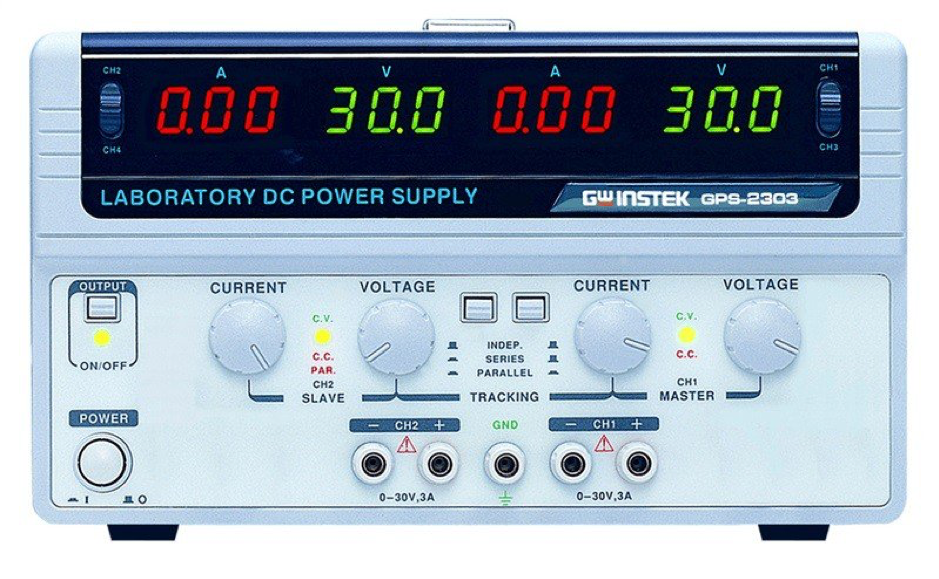
\includegraphics[width=0.7\textwidth]{figures/intro/bench_supply.png}
    \caption{Common laboratory DC power supply \cite{labsupply_price}.}
    \label{fig:bench_supply}
\end{figure}
A typical bench top power supply used within an electronics laboratory is shown in Figure \ref{fig:bench_supply}. Generally, a bench top power supply sources its input voltage from AC mains and makes use of transformer and rectification to step the voltage down to an appropriate DC voltage. To ensure they produce low noise the DC regulation uses linear techniques \cite{benchsupply_specs}. This naturally limits the power supply to only being able to regulate voltages less than the input voltage source. To characterise the performance of a typical power supply, we note: an output range from \SI{0}{V} to \SI{30}{V}, a typical ripple voltage of less than \SI{1}{mV} and low noise. \cite{benchsupply_specs}
\newpar
The inherent problem with power supplies currently are the cost of entry, again looking at a common laboratory supply we see that the typical retail cost can be upwards of \$430 \cite{labsupply_price}. Additionally, they are large and bulky. Both of these factors limit them mainly to already established laboratory environments. With the increase in lower powered portable electronics and the emergence of the Internet of Things (IoT) in recent years, more devices are including embedded microcontrollers in to their products from the start. This brings a strong focus onto software and firmware programming. Being able to start this process early on hardware prototypes and without access to expensive laboratory equipment will help accelerate the design process and bring the product to market faster. 
\newpar
Our solution is a portable bench top power supply, providing a selectable output from \SI{0}{V} to \SI{25}{V} and is capable of supplying \SI{2}{A} peak loads. The device is powered from a single USB port on a computer, requiring no external power supply to use, which increases the portability. It is light, compact and can easily be carried in a bag or placed on a desk taking up minimal space. The user can configure the device easily from a provided interface on a computer, as well as display useful information such as current demand in real time. Furthermore, the device is highly efficient \hl{(provide exact numbers)} and has an output voltage ripple that does not exceed \SI{4.5}{mV} for the entire operating range.  Finally the power supply can continue to supply a regulated output voltage for up to 5 minutes while being disconnected from the USB input. \footnote{See Section \ref{sec:delivered} for product specifications.}
\newpar
This is a unique product as it provides all the functionality of a power supply, however does so in a manner that is portable and in a small footprint.
%%%%%%%%%%%%%%%%%%%%%%%%%%%%%%%%%%%%%%%%%%%%%%%%%%%%%%%%%%%%%%%%%%%%%%%%%%%%%%%%
\subsubsection{Benchmarks}
\subsubsection{USB}
electrical characteristics: maximum $500 \myunit{mA}$ @ fixed $5 \myunit{V}$ DC ($5 \myunit{W}$ power handling)
\subsubsection{Benchtop power supply - GW Instek GPS-2303}
electrical characteristics: maximum $3 \myunit{A}$ @ variable $0 - 30 \myunit{V}$ DC ($90 \myunit{W}$ power handling)
~\\
physical characteristics: product weight $7 \myunit{kg}$; $\sim 0.01 \myunit{m}^3$
~\\
Maybe cost? 430 for the one we have in the lab:  https://core-electronics.com.au/laboratory-dc-power-supply-2x-outputs-at-0-30v-3a.html
%%%%%%%%%%%%%%%%%%%%%%%%%%%%%%%%%%%%%%%%%%%%%%%%%%%%%%%%%%%%%%%%%%%%%%%%%%%%%%%%
%%%%%%%%%%%%%%%%%%%%%%%%%%%%%%%%%%%%%%%%%%%%%%%%%%%%%%%%%%%%%%%%%%%%%%%%%%%%%%%%
\subsection{Background Theory - The 2 subsystems of a charge management system}
\subsubsection{An introduction to DC-DC converters}
\hl{Need to include a line that motivates the DC-DC converter, why can't linear techniques be used - need to step in the input voltage up}
Switched-mode DC-DC converters provide a method for converting a DC input voltage to a DC output voltage of greater or lesser magnitude by the use of 3 fundamental components: a switch; a diode; and an energy storage component. This energy storage component may achieve its function through storage in magnetic field (i.e. inductors) or through storage in electric field (i.e. capacitors). MOSFETs are typically used to achieve the switching behaviour.
\newpar
A sub-class of DC-DC converters are those that can produce an output voltage that is either greater (termed `boost' behaviour) or lesser (termed `buck' behaviour) in magnitude than the input voltage. Such converters are termed `buck-boost' converters. The nature of the switching signal applied to the buck-boost converter determines the mode of operation and is typically of pulse-width modulation (PWM) form. For a typical converter, a PWM signal that is on for a shorter proportion of time than it is off produces buck behaviour and a PWM signal that is on for a longer proportion of time than it is off produces boost behaviour.
\newpar
Buck-boost converters are favoured for their very high efficiency and simplicity of implementation. They exist nearly everywhere where an output DC voltage of greater or lesser magnitude than a DC input voltage is required to be generated.
\newpar
\hl{TODO lead-in paragraph}
%%%%%%%%%%%%%%%%%%%%%%%%%%%%%%%%%%%%%%%%%%%%%%%%%%%%%%%%%%%%%%%%%%%%%%%%%%%%%%%%
\subsubsection{An introduction to ultra-capacitors}
Electrochemical double layer capacitor(EDLCs) is also known as ultra-capacitor or super capacitor. It is a type of capacitor with higher power density than conventional capacitor and higher energy density than batteries. Due to such high capacitance, ultra-capacitors are used as energy storage in applications \cite{maxwell}, \cite{murata}. 

An ultra-capacitor is typically composed of two electrodes coated with activated carbon powder, electrolytes and a separator in between them. Due to activated carbon, they have much bigger surface area allowing more energy to be stored. 

In comparison to batteries, ultra-capacitors have much smaller Equivalent Series Resistance (ESR). This allows high current charging and discharging as well as high power density. So ultra-capacitors are suitable for low power and high power applications, whereas batteries only suitable for low power applications. Due to such high power density, the size of ultra-capacitor is much smaller. However, as a result of low ESR, the stored energy will be released quickly when short-circuited and might cause electric arcing \cite{murata}. Hence care must be taken to limit the current. 

\begin{figure}[h]
    \centering
    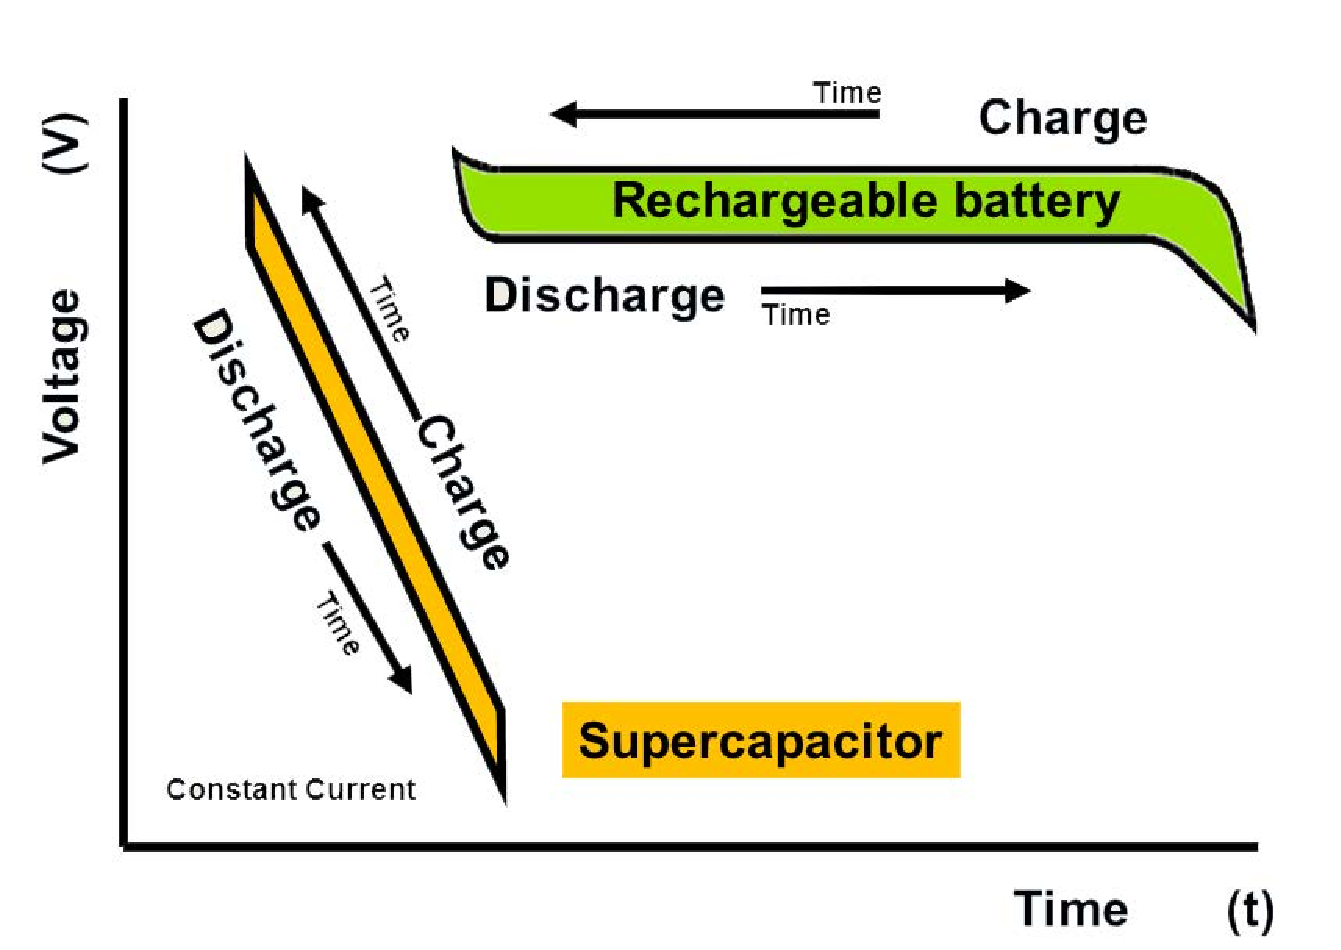
\includegraphics[width=0.7\textwidth]{figures/ultracap_battery.pdf}
    \caption{Ultra-capacitor vs Battery \cite{ultracap_fig}}
    \label{fig:comparison}
\end{figure}

Like a battery, ultra-capacitors also have voltage limits. It can only withstand low voltage, usually 2.7V. Larger voltage can be applied when capacitors are connected in series however balancing is required as over-voltage protection. 

While battery remains at approximately constant voltage until they are depleted, the voltage across ultra-capacitor decreases linearly when a constant current is drawn, refer to Figure \ref{fig:comparison}. Hence additional circuitry to maintain constant voltage is required for ultra-capacitor to act as a battery.

%%%%%%%%%%%%%%%%%%%%%%%%%%%%%%%%%%%%%%%%%%%%%%%%%%%%%%%%%%%%%%%%%%%%%%%%%%%%%%%%
%%%%%%%%%%%%%%%%%%%%%%%%%%%%%%%%%%%%%%%%%%%%%%%%%%%%%%%%%%%%%%%%%%%%%%%%%%%%%%%%
\subsection{What a solution would look like}\label{sec:objectives}
In general terms a solution to the problem as stated in Section~\ref{sec:problem} would comprise ultra-capacitors and charging circuitry, a DC-DC converter circuit connecting ultra-capacitors to a load, and a microcontroller to handle the control regime and communication. The user interface would be achieved through a graphical user interface on a computer connected to the product.
\paragraph{Where power comes from}
Power to run DC-DC converter and all peripheral circuitry should be provided by USB when connected to USB and the ultra-capacitors when not
\paragraph{How communication occurs}
Product should be capable of 2-way communication over USB
\paragraph{What quantity is controlled and where the control occurs \hl{TODO specific performance requirements (overshoot etc.)}}
The control regime should operate on the DC-DC converter circuit output voltage. Control algorithm should be hard-coded into microcontroller with routines for the user to update the reference without re-programming.
\newpar
Output voltage should produce smooth transient behaviour in response to step changes in reference; zero steady-state error; complete rejection of ramp disturbance at converter input (i.e. reject linear decrease in ultra-capacitor voltage as discharging).
\paragraph{What measured \hl{TODO mention GUI also}}
Microcontroller should be hard-coded to send to the user interface the ultra-capacitor stack voltage, DC-DC converter output voltage, control signal, and estimates for state variables.
%%%%%%%%%%%%%%%%%%%%%%%%%%%%%%%%%%%%%%%%%%%%%%%%%%%%%%%%%%%%%%%%%%%%%%%%%%%%%%%%
%%%%%%%%%%%%%%%%%%%%%%%%%%%%%%%%%%%%%%%%%%%%%%%%%%%%%%%%%%%%%%%%%%%%%%%%%%%%%%%%
\subsection{The delivered product}\label{sec:delivered}
\subsubsection{Pictures}
\subsubsection{System diagram}
\subsubsection{Control flow}
\tikzstyle{block} = [rectangle, draw, fill = \myblue, 
text width = 5em, align = center, rounded corners, minimum height = 4em]
\tikzstyle{smallblock} = [rectangle, draw, fill = \myblue, 
text width = 3em, align = center, rounded corners, minimum height = 3em]
\tikzstyle{line} = [draw, -latex']
\begin{figure}[H]
\centering
\fbox{
\begin{tikzpicture}[node distance = 2cm]
    \node [block, fill = \myorange, minimum width = 8em, text width = 8em] (plant) {\textbf{PLANT} \\ DC-DC converter};
    % \node [block, right = of plant, fill = \myblue] (load) {load};
    \node [block, left = of plant, fill = \myblue, minimum width = 9em, text width = 9em] (controller) {\textbf{CONTROLLER} \\ microcontroller \\ integral action};
    \draw ($(controller) + (-3,0)$) node [sum] (s1) {\suma};
    %
    \path [line, ultra thick] ($(s1) + (-1.5,0)$)
    --
    node [anchor = south, align = center, pos = 0.7]
    {$-$}
    (s1);
    %
    \path [line, ultra thick] (s1)
    -- (controller);
    %
    \path [line, ultra thick] (controller)
    --
    node [anchor = south, align = center]
    {duty \\ ratio}
    (plant);
    %
    \path [line, ultra thick] (plant)
    -- ($(plant) + (3,0)$);
    %
    \path [line, ultra thick] ($(plant) + (2.25,0)$)
    -- ($(plant) + (2.25,-2)$)
    -- ($(s1) + (0,-2)$)
    --
    node [anchor = east, align = center, pos = 0.9]
    {$+$}
    (s1);
    %
    \draw ($(s1) + (-2.5,0)$) node [align = center] (ref) {reference \\ voltage};
    \draw ($(plant) + (3.75,0)$) node [align = center] (out) {output \\ voltage};
\end{tikzpicture}
}
\caption{Control flow diagram of product}
\label{fig:controlflow0}
\end{figure}
\subsubsection{Specifications}
physical characteristics: $\sim 0.4 \myunit{kg}$; $\sim 0.0006 \myunit{m}^3$
\begin{itemize}
    \item transient performance
\end{itemize}
%%%%%%%%%%%%%%%%%%%%%%%%%%%%%%%%%%%%%%%%%%%%%%%%%%%%%%%%%%%%%%%%%%%%%%%%%%%%%%%%
%%%%%%%%%%%%%%%%%%%%%%%%%%%%%%%%%%%%%%%%%%%%%%%%%%%%%%%%%%%%%%%%%%%%%%%%%%%%%%%%
\begin{comment}
\subsection{Project Aim}
\begin{itemize}
    \item Ultra-capacitor charge and discharge characteristics must be well described
    \item DC-DC converter must reject ramp disturbances entering at the input voltage
    \item control loop must produce zero steady-state error from reference
    \item system must be safe under normal and extreme operating operating conditions
    \item control loop must be robust
    \item entire system must be charged/powered, and communicate through USB
\end{itemize}
\end{comment}
%%%%%%%%%%%%%%%%%%%%%%%%%%%%%%%%%%%%%%%%%%%%%%%%%%%%%%%%%%%%%%%%%%%%%%%%%%%%%%%%
%%%%%%%%%%%%%%%%%%%%%%%%%%%%%%%%%%%%%%%%%%%%%%%%%%%%%%%%%%%%%%%%%%%%%%%%%%%%%%%%
%%%%%%%%%%%%%%%%%%%%%%%%%%%%%%%%%%%%%%%%%%%%%%%%%%%%%%%%%%%%%%%%%%%%%%%%%%%%%%%%